\begin{frame}{Who? - Lecturers and Tutors}

	%Dominik Probst
	\begin{columns}[T]
		\begin{column}{0.2\textwidth}
			\vspace{-1em}
			\begin{figure}[t]
				\centering
				\includegraphics[width=0.55\textwidth]{img/dominik_probst.jpg}
			\end{figure}
		\end{column}
		\begin{column}{0.6\textwidth}
			\textbf{Dominik Probst, M.Sc.} \\
			\textit{Lecturer, Tutor and Primary Contact}
			\begin{itemize}
				\item Ph.D. candidate \href{https://www.cs6.tf.fau.eu}{@CS6 (Data Management)}
				\item E-Mail: \texttt{\href{mailto:dominik.probst@fau.de}{dominik.probst@fau.de}}
				\item Website: \url{https://www.cs6.tf.fau.eu/dp}
			\end{itemize}
		\end{column}
		\begin{column}{0.2\textwidth}
			\hfill
		\end{column}
	\end{columns}

	\vspace{0.5em}
	{\color{lightgray}\hrule}
	\vspace{1em}

	%Lucas Weber
	\begin{columns}[T]
		\begin{column}{0.2\textwidth}
			\hfill
		\end{column}
		\begin{column}{0.6\textwidth}
			\textbf{Lucas Weber, Dipl.Ing.} \\
			\textit{Tutor}
			\begin{itemize}
				\item Ph.D. candidate \href{https://www.cs6.tf.fau.eu}{@CS6 (Data Management)}
				\item E-Mail: \texttt{\href{mailto:lucas.weber@fau.de}{lucas.weber@fau.de}}
				\item Website: \url{https://www.cs6.tf.fau.eu/lw}
			\end{itemize}
		\end{column}
		\begin{column}{0.2\textwidth}
			\vspace{-1em}
			\begin{figure}[t]
				\centering
				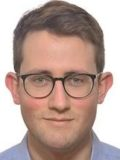
\includegraphics[width=0.55\textwidth]{img/lucas_weber.jpg}
			\end{figure}
		\end{column}
	\end{columns}
\end{frame}

\begin{frame}{For whom? - Courses of Study}
	% Study programs
	\begin{itemize}
		\item \textbf{Knowledge Discovery in Databases with Exercise (KDDmUe)} - 5 ECTS
		      \begin{itemize}
			      \item B.Sc./M.Sc. Data Science
			      \item B.Sc./M.Sc. Computer Science
			      \item M.Sc. International Information Systems
			      \item M.Sc. Medical Engineering
			      \item M.Sc. Information and Communication Technology
			      \item {\color{gray} Possibly other courses of study (clarify with your examination office)}
		      \end{itemize}
	\end{itemize}

	\begin{alertblock}{Important: The \glqq Lecture Only\grqq\ Is No Longer Offered!}
		Until SS2023, we offered the module KDD (2.5 ECTS - only lecture) for some degree programmes. This module is no longer offered!
	\end{alertblock}

\end{frame}

\begin{frame}{For whom? - Prerequisites}
	%Prerequisites
	\begin{itemize}
		\item \textbf{Mandatory requirements:}
		      \begin{itemize}
			      \item Successful completion of the module \glqq Konzeptionelle Modellierung\grqq~(KonzMod)
			            \begin{itemize}
				            \item Or a similar course teaching the basics of databases and SQL
			            \end{itemize}
		      \end{itemize}
		\item \textbf{Useful prerequisites:}
		      \begin{itemize}
			      \item Successful completion of the module \glqq Implementierung von Datenbanksystemen\grqq~(IDB)
			      \item Experience with:
			            \begin{itemize}
				            \item Python
				            \item Jupyter Notebooks
				            \item Numpy
				            \item Pandas
				            \item Algorithms
				            \item Data structures
			            \end{itemize}
		      \end{itemize}
	\end{itemize}

\end{frame}


\begin{frame}{What? - Goal and Topics}
	% Goal of the lecture
	\begin{itemize}
		\item \textbf{Goal of the module:}
		      \begin{itemize}
			      \item Introduce you to the principles of data mining. \\
			            $\Rightarrow$ This is the core of knowledge discovery in databases
		      \end{itemize}
		\item \textbf{Topics in the lecture:}
		      \vspace*{-1\multicolsep}
		      \begin{multicols}{2}
			      \begin{enumerate}
				      \item Introduction
				      \item Data
				      \item Preprocessing
				      \item Data Warehousing
				      \item Mining Frequent Patterns
				      \item Classification
				      \item Cluster Analysis
				      \item Outlier Analysis
				            %\item {\color{gray}Guest lecture} \\
				            %      {\color{gray}(Not part of the exam)}
			      \end{enumerate}
		      \end{multicols}
		      \vspace*{-0.75\multicolsep}
		\item \textbf{Topics in the exercise:}
		      \vspace*{-1\multicolsep}
		      \begin{multicols}{2}
			      \begin{enumerate}
				      \item Introduction to python and pandas {\color{gray}(optional)}
				      \item Data Analysis and Data Preprocessing
				      \item Frequent Patterns
				      \item Classification
				      \item Clustering
				      \item Outlier
			      \end{enumerate}
		      \end{multicols}
		      \vspace*{-0.75\multicolsep}
		\item \textbf{Topics in the submissions:}
		      \vspace*{-1\multicolsep}
		      \begin{multicols}{2}
			      \begin{enumerate}
				      \item Frequent Patterns
				      \item Classification
				      \item Clustering
			      \end{enumerate}
		      \end{multicols}
		      \
	\end{itemize}
\end{frame}

\begin{frame}{What? - Exercises}
	\begin{itemize}
		\item \textbf{Exercise sessions (in presence):}
		      \begin{itemize}
			      \item Working together on exercise sheets
			      \item Either practical data science tasks or theoretical exercises \\
			            {\color{gray}(varies depending on the exercise sheet)}
			      \item Required tools:
			            \begin{itemize}
				            \item Laptop capable of running Jupyter Notebooks \\
				                  {\color{gray}(preferably one per person, one per small group is also possible)}
			            \end{itemize}
			      \item Expected preparation:
			            \begin{itemize}
				            \item Good understanding of the lecture content
				            \item Completed "Preparation" section (see exercise sheets)
			            \end{itemize}
		      \end{itemize}
	\end{itemize}
\end{frame}

\begin{frame}{Why? - Exercises}
	\begin{itemize}
		\item \textbf{Last semester:}
		      \begin{itemize}
			      \item Very low attendance in the exercise sessions (below 5\% of registered students)\\
			            $\Rightarrow$ Tasks \underline{based on} the exercise sheets with very low point averages in the exam
		      \end{itemize}
	\end{itemize}

	\only<2->{
		\begin{center}
			\scalebox{0.75}{
				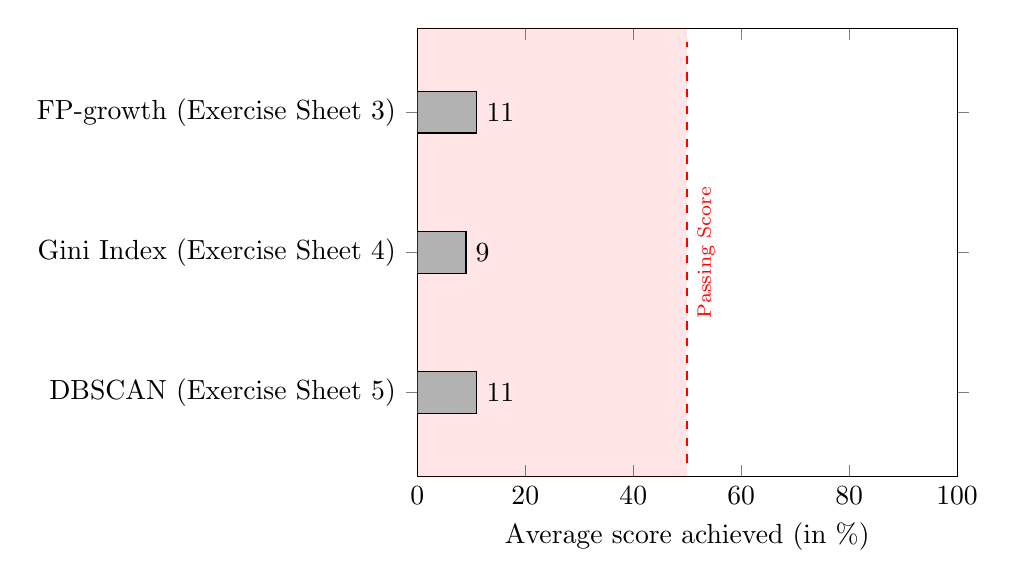
\begin{tikzpicture}
					\begin{axis}[
						xbar,
						xmin=0, xmax=100,
						ytick={0, 1, 2},
						yticklabels={
						DBSCAN {(Exercise Sheet 5)},
						Gini Index {(Exercise Sheet 4)},
						FP-growth {(Exercise Sheet 3)},
						},
						xlabel={Average score achieved (in \%)},
						nodes near coords,
						bar width=15pt,
						enlarge y limits=0.3,
						]

						\draw[fill=red, fill opacity=0.1, draw=none] (0,-0.6) rectangle (axis cs:50,2.6);

						\addplot [fill=gray!60] coordinates {
								(11,0) 	% DBSCAN
								(9,1)	% Gini Index
								(11,2) 	% FP-growth
							};


						\draw [red, thick, dashed]
						(axis cs:50,-0.5) -- (axis cs:50,2.5)
						node[pos=0.5, anchor=north, rotate=90, red] {\scriptsize Passing Score};
					\end{axis}
				\end{tikzpicture}
			}
		\end{center}
	}

	\only<3->{
		\begin{alertblock}{Important: The Exercises Are Crucial For The Exam!}
			While the lectures give you a basic theoretical overview, the exercises go into more detail, give you some more practical insights, and will be the basis of multiple questions in the exam!
		\end{alertblock}
	}

\end{frame}

\begin{frame}{What? - Submissions}
	\begin{itemize}
		\item \textbf{Programming tasks (to be done at home):}
		      \begin{itemize}
			      \item Implementation of individual algorithms known from the lecture for a deeper understanding \\
			            \begin{itemize}
				            \item Programming language: Python
				            \item Topics: Frequent Patterns, Classification, and Clustering
			            \end{itemize}
			      \item Have to be submitted to a GitHub classroom
			            \begin{itemize}
				            \item Calculation of points performed automatically after each push
				            \item Improvements possible at any time until the submission deadline
			            \end{itemize}
			      \item Work in small groups (up to three persons) is permitted
			            \begin{itemize}
				            \item We conduct random checks for plagiarism across groups \\
				                  $\Rightarrow$ In cases where plagiarism is detected, all groups involved will receive zero points.
			            \end{itemize}
		      \end{itemize}
		      \begin{block}{Participating In Or Passing The Submissions Is Not Mandatory!}
			      However, if you get \underline{at least 50\%} of the points, you will receive access to a mock exam with solutions. \\
			      Also some exam questions \underline{will be} easier to solve if you have completed the submissions.
		      \end{block}
	\end{itemize}
\end{frame}

\begin{frame}{What? - Exam}
	% Exam
	\begin{itemize}
		\item \textbf{Knowledge Discovery in Databases with Exercise (KDDmUe)} - {\color{faugray}Written Exam}
		      \begin{itemize}
			      \item Duration: 90 minutes
			      \item Questions about lecture, exercise \underline{and} submission content
			      \item Language: English
		      \end{itemize}
	\end{itemize}
	\begin{alertblock}{Important: Do Not Forget To Register!}
		Without exception, we can only examine participants who have also registered for this exam at the examination office. Please note the information of the examination office as to when registration takes place in this semester.
	\end{alertblock}
\end{frame}

\begin{frame}{What? - Literature}
	% Literature
	\begin{itemize}
		\item \textbf{This lecture is based on the book by \citeauthor{han2011}:}
		      \begin{itemize}
			      \item \fullcite{han2011}
			      \item {\color{faugray}Copies are available at the Science and Technology Branch Library (TNZB).}
			      \item Lecture slides are based on slides provided by Jiawei Han with modifications by Prof. Dr.-Ing. Klaus Meyer-Wegener and Luciano Melodia.
			      \item Lecture slides have been modified and extended a lot since then.
		      \end{itemize}
		\item \textbf{Further books on this topic include, but not limited to:}
		      \begin{itemize}
			      \item \fullcite{geron2017}
			      \item \fullcite{du2010}
			      \item \fullcite{witten2016}
		      \end{itemize}
	\end{itemize}
\end{frame}

\begin{frame}{When? - Dates}
	% Dates
	\begin{columns}
		\begin{column}{0.5\textwidth}
			\begin{itemize}
				\item \textbf{Lecture} - Start in Calendar Week 17 (Today)
				      \begin{itemize}
					      \item Monday, 14:15 - 15:45 (H20) \\
					            {\color{gray}Lecturer: Dominik Probst}
				      \end{itemize}
			\end{itemize}
		\end{column}

		\begin{column}{0.5\textwidth}
			\begin{itemize}
				\item \textbf{Exercises} - Start in Calendar Week 18
				      \begin{itemize}
					      \item Group 1: Tuesday, 10:15 - 11:45 (H18) \\
					            {\color{gray}Tutor: Lucas Weber}
					      \item Group 2: Wednesday, 16:15 - 17:45 (H4) \\
					            {\color{red}Not offered this semester}
					      \item Group 3: Wednesday, 08:15 - 09:45 (H4) \\
					            {\color{gray}Tutor: Dominik Probst}
					      \item Group 4: Monday, 14:15 - 15:45 (H5) \\
					            {\color{red}Not offered this semester}
				      \end{itemize}
			\end{itemize}
		\end{column}
	\end{columns}

	\begin{block}{Registration For The Exercises}
		Registration for exercises is mandatory to ensure an appropriate support to questions regarding setting of exercises should they arise.
			{\color{faured}Registration opens at April 23th, 16:00 via StudOn.}
	\end{block}
\end{frame}

\begin{frame}{When? - Preliminary Schedule}
	% Schedule
	\footnotesize
	\centering
	\begin{tabular}{|p{4em}|p{15em}|p{9.5em}|p{9.5em}|p{10em}|}
		\hline
		\rowcolor{faugray!62}\textbf{Calendar Week} & \textbf{Lecture}                  & \multicolumn{2}{|l|}{\textbf{Exercise}}                                         & \textbf{Submission}                                \\ \hhline{*{5}{:=}:}
		\cellcolor{faugray!25}17                    & Prologue + Introduction           & \multicolumn{2}{|l|}{\cellcolor{gray!50}}                                       & \cellcolor{gray!50}                                \\ \hhline{|-|-|--|-|}
		\cellcolor{faugray!25}18                    & Data                              & \multicolumn{2}{|c|}{Introduction to Python \& pandas {\color{gray}(optional)}} & \cellcolor{gray!50}                                \\ \hhline{|-|-|--|-|}
		\cellcolor{faugray!25}19                    & \multirow{2}{*}{Preprocessing}    & \multicolumn{2}{|c|}{\multirow{3}{*}{Data Analysis \& Data Preprocessing}}      & \cellcolor{gray!50}                                \\ \hhline{|-|~|~~|-|}
		\cellcolor{faugray!25}20                    &                                   & \multicolumn{2}{|l|}{}                                                          & \cellcolor{gray!50}                                \\ \hhline{|-|-|~~|-|}
		\cellcolor{faugray!25}21                    & Data Warehousing                  & \multicolumn{2}{|l|}{}                                                          & \cellcolor{gray!50}                                \\ \hhline{|-|-|--|-|}
		\cellcolor{faugray!25}22                    & \multirow{2}{*}{Frequent Pattern} & \multicolumn{2}{|c|}{\cellcolor{gray!50}}                                       & \cellcolor{gray!50}                                \\ \hhline{|-|~|--|-|}
		\cellcolor{faugray!25}23                    &                                   & \multicolumn{2}{|c|}{Frequent Pattern {\color{gray}(Part 1)}}                   & \cellcolor{gray!50}                                \\ \hhline{|-|-|--|-|}
		\cellcolor{faugray!25}24                    & \multirow{2}{*}{Classification}   & \multicolumn{2}{|l|}{\cellcolor{gray!50}}                                       & \cellcolor{gray!50}                                \\ \hhline{|-|~|~~|-|}
		\cellcolor{faugray!25}25                    &                                   & \multicolumn{2}{|c|}{Frequent Pattern {\color{gray}(Part 2)}}                   & \multirow{2}{*}{\cellcolor{white}Frequent Pattern} \\ \hhline{|-|-|--|~|}
		\cellcolor{faugray!25}26                    & \multirow{2}{*}{Cluster Analysis} & \multicolumn{2}{|c|}{\multirow{3}{*}{Classification}}                           &                                                    \\ \hhline{|-|~|~~|-|}
		\cellcolor{faugray!25}27                    &                                   & \multicolumn{2}{|l|}{}                                                          & \multirow{2}{*}{\cellcolor{white}Classification}   \\ \hhline{|-|-|~~|~|}
		\cellcolor{faugray!25}28                    & \multirow{2}{*}{Outlier Analysis} & \multicolumn{2}{|l|}{}                                                          &                                                    \\ \hhline{|-|~|--|-|}
		\cellcolor{faugray!25}29                    &                                   & \multicolumn{2}{|c|}{\multirow{2}{*}{Clustering}}                               & \multirow{2}{*}{\cellcolor{white}Clustering}       \\ \hhline{|-|-|~~|~|}
		\cellcolor{faugray!25}30                    & Exam Q\&A                         & \multicolumn{2}{|l|}{}                                                          &                                                    \\ \hline
	\end{tabular}

\end{frame}

\begin{frame}{Where? - StudOn}
	% StudOn
	\begin{columns}
		\begin{column}{0.7\textwidth}
			\begin{itemize}
				\item Register at: \url{https://www.studon.fau.de/crs5533883_join.html}
				\item Main source for resources. E.g.:
				      \begin{itemize}
					      \item Lecture slides
					      \item Exercise sheets
					      \item Forum
				      \end{itemize}
				\item Membership required to receive important updates on KDD by mail
				\item Questions should be asked here (StudOn Forum)

			\end{itemize}
		\end{column}
		\begin{column}{0.3\textwidth}
			\begin{center}
				\qrcode{https://www.studon.fau.de/crs5533883_join.html}
			\end{center}
		\end{column}
	\end{columns}

\end{frame}


\begin{frame}{Where? - GitHub}
	% GitHub
	\begin{columns}
		\begin{column}{0.7\textwidth}
			\begin{itemize}
				\item Public repository at: \url{https://github.com/FAU-CS6/KDD}
				\item Version control of our resources including:
				      \begin{itemize}
					      \item Lecture slides
					      \item Exercise sheets
				      \end{itemize}
			\end{itemize}
		\end{column}
		\begin{column}{0.3\textwidth}
			\begin{center}
				\qrcode{https://github.com/FAU-CS6/KDD}
			\end{center}
		\end{column}
	\end{columns}
	\vspace{5mm}
	\begin{exampleblock}{Help Appreciated: Error Corrections}
		Even though we strive for error-free lecture slides and practice sheets, there is still the possibility  that errors have slipped in. You can help us mitigate these inaccuracies: Mail us, or better yet, in the case you have a GitHub account, open up a GitHub issue or create a pull request. Any pointers to errors are very much appreciated.
	\end{exampleblock}

\end{frame}
